
\newpage

\subsection{}
Consider the graph of
$$y={1\over\sqrt{1+x^2}}$$
over the domain from 0 to infinity.
The following graph demonstrates the general idea.

\medskip
\verb$xrange=(0,10)$

\verb$yrange=(-1,1)$

\verb$draw(1/sqrt(1+x^2))$

\begin{center}
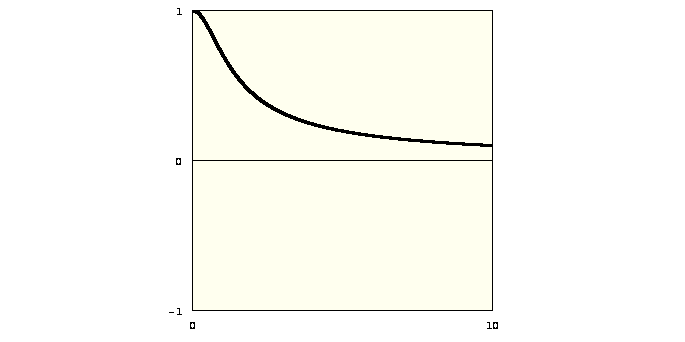
\includegraphics[scale=0.4]{16.png}
\end{center}

\medskip
\noindent
Now imagine that the graph is rotated about the $x$ axis.
What is the volume subtended by the area under the curve?

\medskip
\noindent
To solve, use cylindrical coordinates.
The $x$ axis becomes the $z$ axis.
We want $x$ to become a function of $y$ so invert the function.
$$y={1\over\sqrt{1+x^2}}
\quad\rightarrow\quad
{1\over y^2}=1+x^2
\quad\rightarrow\quad
x=\sqrt{{1\over y^2}-1}
$$

